% Arquivo LaTeX de exemplo de disserta?o/tese a ser apresentados à CPG do IME-USP
%
% Vers? 5: Sex Mar  9 18:05:40 BRT 2012
%
% Cria?o: Jesus P. Mena-Chalco
% Revisão: Fabio Kon e Paulo Feofiloff
%
% Obs: Leia previamente o texto do arquivo README.txt

\documentclass[11pt,twoside,a4paper]{book}

% ---------------------------------------------------------------------------- %
% Pacotes
\usepackage{fontspec}
\usepackage{polyglossia}
\setdefaultlanguage{brazil}

\usepackage{graphicx}           % usamos arquivos pdf/png como figuras
\usepackage{setspace}                   % espaçamento flexível
\usepackage{indentfirst}                % indenta?o do primeiro par?rafo
\usepackage{makeidx}                    % ?dice remissivo
\usepackage[nottoc]{tocbibind}          % acrescentamos a bibliografia/indice/conteudo no Table of Contents
\usepackage{courier}                    % usa o Adobe Courier no lugar de Computer Modern Typewriter
\usepackage{type1cm}                    % fontes realmente escal?eis
\usepackage{listings}                   % para formatar código-fonte (ex. em Java)
\usepackage{titletoc}
%\usepackage[bf,small,compact]{titlesec} % cabe?lhos dos t?ulos: menores e compactos

\usepackage[font=small,format=plain,labelfont=bf,up,textfont=it,up]{caption}
\usepackage[usenames,svgnames,dvipsnames]{xcolor}
\usepackage[a4paper,top=2.54cm,bottom=2.0cm,left=2.0cm,right=2.54cm]{geometry} % margens
%\usepackage[pdftex,plainpages=false,pdfpagelabels,pagebackref,colorlinks=true,citecolor=black,linkcolor=black,urlcolor=black,filecolor=black,bookmarksopen=true]{hyperref} % links em preto
\usepackage[plainpages=false,pdfpagelabels,pagebackref,colorlinks=true,citecolor=DarkGreen,linkcolor=NavyBlue,urlcolor=DarkRed,filecolor=green,bookmarksopen=true]{hyperref} % links coloridos
\usepackage[all]{hypcap}                % soluciona o problema com o hyperref e capitulos
\usepackage[square,sort,nonamebreak,comma]{natbib}  % cita?o bibliogr?ica alpha (alpha-ime.bst)
\fontsize{60}{62}\usefont{OT1}{cmr}{m}{n}{\selectfont}

% ---------------------------------------------------------------------------- %
% Cabe?lhos similares ao TAOCP de Donald E. Knuth
\usepackage{fancyhdr}
\pagestyle{fancy}
\fancyhf{}
\renewcommand{\chaptermark}[1]{\markboth{\MakeUppercase{#1}}{}}
\renewcommand{\sectionmark}[1]{\markright{\MakeUppercase{#1}}{}}
\renewcommand{\headrulewidth}{0pt}

% ---------------------------------------------------------------------------- %
\graphicspath{{./figuras/}}             % caminho das figuras (recomend?el)
\frenchspacing                          % arruma o espa?: id est (i.e.) e exempli gratia (e.g.)
\urlstyle{same}                         % URL com o mesmo estilo do texto e n? mono-spaced
\makeindex                              % para o ?dice remissivo
\raggedbottom                           % para n? permitir espa?s extra no texto
\fontsize{60}{62}\usefont{OT1}{cmr}{m}{n}{\selectfont}
\cleardoublepage
\normalsize

% ---------------------------------------------------------------------------- %
% Op?es de listing usados para o c?igo fonte
% Ref: http://en.wikibooks.org/wiki/LaTeX/Packages/Listings
\lstset{ %
language=Java,                  % choose the language of the code
basicstyle=\footnotesize,       % the size of the fonts that are used for the code
numbers=left,                   % where to put the line-numbers
numberstyle=\footnotesize,      % the size of the fonts that are used for the line-numbers
stepnumber=1,                   % the step between two line-numbers. If it's 1 each line will be numbered
numbersep=5pt,                  % how far the line-numbers are from the code
showspaces=false,               % show spaces adding particular underscores
showstringspaces=false,         % underline spaces within strings
showtabs=false,                 % show tabs within strings adding particular underscores
frame=single,	                % adds a frame around the code
framerule=0.6pt,
tabsize=2,	                    % sets default tabsize to 2 spaces
captionpos=b,                   % sets the caption-position to bottom
breaklines=true,                % sets automatic line breaking
breakatwhitespace=false,        % sets if automatic breaks should only happen at whitespace
escapeinside={\%*}{*)},         % if you want to add a comment within your code
backgroundcolor=\color[rgb]{1.0,1.0,1.0}, % choose the background color.
rulecolor=\color[rgb]{0.8,0.8,0.8},
extendedchars=true,
xleftmargin=10pt,
xrightmargin=10pt,
framexleftmargin=10pt,
framexrightmargin=10pt
}

% ---------------------------------------------------------------------------- %
% Corpo do texto
\begin{document}
\frontmatter
% cabe?lho para as p?inas das se?es anteriores ao cap?ulo 1 (frontmatter)
\fancyhead[RO]{{\footnotesize\rightmark}\hspace{2em}\thepage}
\setcounter{tocdepth}{2}
\fancyhead[LE]{\thepage\hspace{2em}\footnotesize{\leftmark}}
\fancyhead[RE,LO]{}
\fancyhead[RO]{{\footnotesize\rightmark}\hspace{2em}\thepage}

\onehalfspacing  % espa?mento

% ---------------------------------------------------------------------------- %
% CAPA
% Nota: O t?ulo para as disserta?es/teses do IME-USP devem caber em um
% orif?io de 10,7cm de largura x 6,0cm de altura que h?na capa fornecida pela SPG.
\thispagestyle{empty}
\begin{center}
    \vspace*{2.3cm}
    \textbf{\Large{Implantação de um programa de Engenharia de Software em uma empresa de desenvolvimento de software}}\\

    \vspace*{1.2cm}
    \Large{Alex Tito de Morais}\\
    \Large{Marcelo de Rezende Martins}

    \vskip 0.5cm
    \normalsize{\today}
\end{center}






% ---------------------------------------------------------------------------- %
% Resumo
\chapter*{Resumo}

\noindent  \textbf{Estudo de caso: Restaurante \textit{Da Gino}}.\\



Estudo de caso do Restaurante \textit{Da Gino}. Neste trabalho exibiremos como o Scrum e métodos ágeis aplicam-se como modelo de processo segundo as atividades da ISO 12207:1995.\\ 



\noindent \textbf{Palavras-chave:} scrum, métodos ágeis, iso 12207.



% ---------------------------------------------------------------------------- %
% Sumário
\tableofcontents    % imprime o sumário



% ---------------------------------------------------------------------------- %
% Listas de figuras e tabelas criadas automaticamente
\listoffigures
\listoftables

% ---------------------------------------------------------------------------- %
% Cap?ulos do trabalho
\mainmatter

% cabeçalho para as páinas de todos os capítulos
\fancyhead[RE,LO]{\thesection}

\singlespacing              % espaçamento simples
%\onehalfspacing            % espaçamento um e meio

%% ------------------------------------------------------------------------- %%
\chapter{Introdução}
\label{cap:introducao}

\section{Escopo}

O presente trabalho visa apresentar as decisões e o conjunto de propostas que irão orientar a estratégia de implantação de um programa de Engenharia de Software em uma empresa de desenvolvimento de software fictícia. Esta empresa será responsável pelo desenvolvimento de um software que atenda ao escopo apresentado no estudo de caso \textit{"Restaurante Da Gino"}.

\subsection{Premissas assumidas}

\emph{"O Gino quer abrir um restaurante: o Da Gino, com grande capacidade de lugares, pretendendo informatizar alguns aspectos do seu negócio. Sua experiência no ramo mostrou que é preciso padronizar as receitas das refeições, ter um bom controle do consumo dos itens utilizados na preparação das refeições e ter agilidade no controle da disponibilidade das mesas. A informatização deverá ajudar o cumprimento desses objetivos de negócio, pois o Gino pretende operar com uma equipe pequena de funcionários."}\\
\textbf{Local}: Novo\\
\textbf{Funcionários}: 20 funcionários incluindo o Gino

%% ------------------------------------------------------------------------- %%
\section{Organização do documento}
\label{sec:organizacao_trabalho}

No capítulo~\ref{cap:processoengenharia}, apresentamos a proposta de programa de engenharia de software implantado na empresa responsável pelo produto de software definido na disciplina. O capítulo~\ref{cap:processoengenharia} cobre as seguintes áreas de conhecimento:

\begin{enumerate}
	\item Ciclo de vida e modelo de processo~\ref{sec:modelodeprocesso}
	\item Requisitos de software~\ref{sec:requisitos}
	\item Qualidade de software~\ref{sec:qualisoftware}
	\item Gerência da engenharia de software~\ref{sec:gerenciaengenharia}
	\item Gerência da configuração de software~\ref{sec:gerenciaconfig}
	\item Teste de software~\ref{sec:teste}
\end{enumerate}

 E no capítulo~\ref{cap:conclusoes} apresentamos as considerações finais sobre o trabalho e a disciplina.


        % associado ao arquivo: 'cap-introducao.tex'
%% ------------------------------------------------------------------------- %%
\chapter{Processo de engenharia de software}
\label{cap:processoengenharia}

Processo de Engenharia de Software é uma sequência coerente de práticas que objetiva o desenvolvimento ou evolução de sistemas de software. Estas práticas englobam as atividades de especificação, projeto, desenvolvimento, testes e caracterizam-se pela interação de ferramentas, pessoas e métodos \cite{engsoftiki:17}.

O processo de engenharia de software corresponde à definição, desenvolvimento, medição, gerenciamento, mudança e melhoria dos próprios processos de software \cite{SWEBOK2004}.

A definição de processo pode ser um procedimento, uma política, ou uma norma. Processos de ciclo de vida de software são definidos por uma série de razões, incluindo o incremento da qualidade do produto, melhorias da compreensão humana e comunicação, apoio ao processo de melhoria, apoio aos processos de gestão, orientação aos processos automatizados, e providenciando a execução de suporte automatizado \cite{SWEBOK2004}. 

Os tipos de definições exigidas no processo dependerão, pelo menos parcialmente, do motivo da definição. Também é importante notar que o contexto do projeto e da organização irão determinar a definição do tipo de processo que é mais útil. Variáveis importantes a considerar incluem a natureza do trabalho (por exemplo, a manutenção ou desenvolvimento), o domínio da aplicação, o modelo do ciclo de vida, e da maturidade da organização. \cite{SWEBOK2004}.

O principal objetivo é apresentar um modelo de processo de software apropriado para o estudo de caso \textit{"Restaurante Da Gino"} a partir da adaptação da ISO/IEC 12207:1995.

\section{Seleção do modelo de processo}

Um modelo de processo de software, ou simplesmente modelo de processo, pode ser visto como uma representação abstrata de um processo de software, apresentando a descrição do processo segundo uma perspectiva particular. Além disso, oferece uma forma mais abrangente e fácil de representar o gerenciamento de processo de software e consequentemente o progresso do projeto \cite{engsoftiki:17}.

O modelo de ciclo de vida que corresponde ao modelo de processo, é uma estrutura contendo processos, atividades e tarefas envolvidas no desenvolvimento, operação e manutenção de um produto de software, abrangendo a vida do sistema desde a definição de seus requisitos até o término de seu uso \cite{iso12207:95}.

Para definir o modelo de processo a ser adotado, foi necessário definir os critérios de seleção e analisá-las sob a perspectiva do adquirente e fornecedor, no caso, restaurante \textit{Da Gino} e a empresa de desenvolvimento de software, respectivamente.


\section{Critérios de seleção do modelo de processo}

Os principais pontos que foram analisados para a escolha do modelo de processo foram os seguintes fatores:

\begin{description}
  \item [Organizacionais] As políticas das organizações em questão, que neste caso seriam a empresa contratada para o desenvolvimento do projeto e o adquirente (Gino);
  \item [Documentação que deve ser gerada para o produto] Analisamos algumas necessidades e também informações disponibilizadas pelo adquirente;
  \item [Características do projeto] Analisamos algumas características do projeto a ser desenvolvido:
  \begin{itemize}
    \item Criticidade
    \item Tamanho
    \item Visibilidade
    \item Prazos de tempo e custo
    \item Requisitos do sistema
  \end{itemize}

\end{description}

\section{Definição do modelo de processo}

O modelo de processo que definimos para o desenvolvimento do software do restaurante \textit{Da Gino} foi um modelo de processo baseado nas características dos modelos ágeis, cujas principais características são um processo iterativo que organiza-se através do desenvolvimento baseado em entregas frequentes em curtos períodos de tempo, e também é guiado por boas práticas para inúmeros processos como documentação, desenvolvimento, comunicação e gerenciamento em geral. Analisando a definição frente a um modelo de ciclo de vida foi escolhido o modelo de processo baseado em métodos ágeis Scrum.

\section{Justificativa para a adoção do Modelo de Processo}

Com relação ao fator organizacional verificou-se que o Restaurante \textit{Da Gino} encontra-se em pré-construção tanto de sua parte física quanto dos processos lógicos que regeriam a organização e como hipótese assumida definimos que os processos de regras organizacionais seriam processos de grande maleabilidade e fácil adaptação. 

A empresa responsável pelo desenvolvimento do sistema é uma fábrica de software e possui como principal regra organizacional o fator produtividade, portanto o desenvolvimento de sistemas é baseado principalmente em entregas frequentes em pequenos intervalos de tempo. 

A partir disto, conclui-se que as duas empresas apresentam uma grande flexibilidade e desejam ter um sistema funcionando em um curto espaço de tempo. 

Já com relação a documentação, assumiremos que os documentos exigidos pelo adquirente são documentos de baixa complexidade e que somente refletem as formas de utilização do sistema, como por exemplo, um manual final de utilização do sistema. Do lado da empresa desenvolvedora em função dos objetivos  finais fica claro que neste caso quanto mais específica for a documentação permitindo que o desenvolvimento seja realizado é o suficiente, ou seja, a documentação precisa auxiliar principalmente o desenvolvimento e não as outras equipes como qualidade, de teste e gerenciamento.

Analisando as principais características do produto a ser desenvolvido, temos:

\begin{description}
  \item [Criticidade e Visibilidade] o software a ser desenvolvido não é um sistema crítico e não será um sistema que irá alavancar o nome de uma empresa, portanto não possui grande visibilidade como produto para o restaurante \textit{Da Gino}. Logo, não há a necessidade de empresas terceiras que avaliem a qualidade, inspecionem os códigos e as funcionalidades ou que valide com extrema cautela através de processos específicos, pois este papel poderá ser realizado pelo própria equipe desenvolvedora.
  \item [Prazos de tempo e custo] Assumiremos que o projeto tem um custo reduzido para ser desenvolvido por volta R\$ 350.000,00 para ser utilizado na compra de equipamentos eletrônicos, computadores, monitores e custear todo o projeto, além disso necessita que seja desenvolvido e terminado com restrições de tempo, cerca de 6 meses. A partir desta premissa, é necessário escolher um modelo de processo que permita desenvolver uma aplicação com uma equipe reduzida de no máximo cinco pessoas, com média a alta experiência e que seja auto-sustentável, organizável, e possuam facilidade na troca de informações.

  \item [Requisitos do sistema] os requisitos do sistema não são complexos, no entanto serão todos passados pelo dono do restaurante que no caso não possui conhecimento nenhum na área de sistemas, portanto concluímos que os requisitos são altamente mutáveis e podem estar incompletos o que irá refletir na equipe de desenvolvimento que por sua vez precisa ser capaz de gerenciar com sucesso às frequentes mudanças dos requisitos.
\end{description}

A partir das análises das principais características do produto, dos aspectos organizacionais e da documentação, concluímos o modelo de processo baseado em metodologias ágeis é o mais adequado. O modelo de processo ágil adotado será o \textit{Scrum}. O princípio chave do \textit{Scrum} é o reconhecimento que os clientes irão mudar de idéia sobre o que eles precisam e querem e que estas mudanças são imprevisíveis. A partir disso, o \textit{Scrum} foca em como maximizar as habilidades do time para fazer entregas mais rápido, para responder a alterações nos requisitos e para adaptar-se ao avanço das tecnologias e mudanças do mercado \cite{scrumwiki:17}.

%% ------------------------------------------------------------------------- %%
\section{Processo de aquisição}
\label{sec:aquisicao}

Segundo a NBR ISO/IEC 12207:1998 \cite{iso12207:95}, o processo de aquisição é composto pelas seguintes atividades:

\begin{enumerate}
  \item Iniciação
  \item Preparação de pedido de proposta
  \item Preparação e atualização do contrato
  \item Monitoração do fornecedor
  \item Aceitação e conclusão
\end{enumerate}

Segundo o item 5.1.1.1 da ISO \cite{iso12207:95}, o adquirente (Gino) inicia o processo com a
descrição de um conceito ou necessidade a adquirir. Principais necessidades do adquirente são:

\begin{itemize}
  \item Padronizar catálogo de receitas
  \item Controle de estoque
  \item Controle de disponibilidade de mesas
\end{itemize}

Segundo o item 5.1.1.4, o adquirente (Gino) pode executar a definição e a análise dos requisitos do software por conta própria ou pode manter acordo com um fornecedor para executar essa tarefa. O adquirente optou por manter um acordo com a empresa de software para que seja feita a definição e análise dos requisitos. Documento de visão será criado para detalhar melhor os requisitos e a estrutura organizacional.



%% ------------------------------------------------------------------------- %%
\section{Processo de fornecimento}
\label{sec:fornecimento}

O fornecedor será responsável por analisar todos os requisitos do sistema de acordo com as necessidades levantadas pelo adquirente (Gino), através de um acordo de contrato. A proposta de tipo de contrato terá escopo variável. Quanto à responsabilidade das organizações, o fornecedor deverá atender as necessidades estabelecidas pelo adquirente para o aceite do software desenvolvido e é de responsabilidade do adquirente prover todas as informações e dados ao fornecedor para a definição do produto final.
O fornecedor será responsável por realizar toda a preparação necessária para elaboração do pedido de proposta do cliente, neste caso, o Gino.

Para a elaboração do pedido de proposta, o fornecedor tem a responsabilidade pelos seguintes itens \cite{iso12207:95}:
\begin{itemize}
  \item Requisitos do sistema
  \item Declaração do escopo
  \item Lista de produtos de software
  \item Termos e condições
  \item Restrições técnicas
\end{itemize}

Após prover os itens acima, eles só serão validados mediante aprovação do cliente.

O contrato será confeccionado mediante direitos de uso, de propriedade, de autoria, de garantia e de licença \cite{iso12207:95}. O adquirente terá prioridade no suporte da aplicação por período pré-estabelecido entre as partes. Também fica pré-definido que qualquer alteração ou aditivo que ocorra no contrato, o fornecedor e o adquirente devem estar em comum acordo. Um documento aprovado por ambas as partes deve ser elaborado suportando estas modificações: análise de impacto quanto a prazos, cronograma e custos \cite{iso12207:95}.

A aceitação será realizada de acordo com o descrito em cada item de requisito levantado, durante as entregas parciais. Uma vez que o fornecedor faz uso de um modelo de desenvolvimento que prevê entregas parciais, o adquirente poderá fazer a validação, verificação e aceitação destas entregas evoluindo até a aceitação final do projeto. A monitoração será realizada de acordo com os status das entregas parciais providas pelo fornecedor. 

Segue a descrição das tarefas e atividades do fornecedor para o processo de fornecimento:


\subsection{Iniciação}

Fornecedor conduzirá uma revisão das necessidades levantadas pelo adquirente para decidir ou propor mudanças para a aceitação do contrato (5.2.1.1 e 5.2.1.2) \cite{iso12207:95}.

\subsection{Preparação de resposta}

O fornecedor será responsável por definir todos os requisitos em resposta ao pedido do \textit{Gino}.

\subsection{Contrato}

Contrato terá escopo variável para atender as necessidades do adquirente de acordo com suas prioridades e trabalhar de acordo com o modelo de desenvolvimento da empresa, Scrum.

\subsection{Planejamento}

\begin{itemize}
  \item Recursos internos para o desenvolvimento do software utilizando o modelo iterativo Scrum (5.2.4.4)
  \item Requisitos e prioridades serão descritos pelo documento de Visão (5.2.4.1)
  \item Estrutura organizacional e cada ciclo será definido pelo Scrum (5.2.4.2 e 5.2.4.5 a.)
  \item Uso do Kanban e diagrama de Burndown para realizar acompanhamento do progresso (5.2.4.5 n.)
  \item Estes diagramas de \textit{Burndown} poderão ser disponibilizados periodicamente ao adquirente para acompanhamento do progresso
  \item Será provido treinamento ao adquirente para a utilização do produto do software (5.2.4.5 o.)
\end{itemize}

\subsection{Execução e controle}

Monitoramento de progresso feito por Kanban e Burndown (5.2.5.3).

\subsection{Revisão e avaliação}

Fornecedor fará uso de um modelo de entregas parciais. O adquirente irá revisar de acordo com a descrição em cada item de requisito levantando durante as entregas parciais. 

\subsection{Entrega e conclusão}

O modelo de processo adotado baseia-se em entregas frequentes de versões do produto que sejam completos e utilizáveis. Quer dizer, o cliente ao final de cada entrega terá uma versão do produto que já pode ser utilizada. O adquirente fará a validação e aceitação das entregas parciais evoluindo até a aceitação do produto final.

%% ------------------------------------------------------------------------- %%
\section{Processo de desenvolvimento}
\label{sec:desenvolvimento}

Segue uma descrição das atividades e tarefas do processo de desenvolvimento:

\subsection{Implementação do processo}

O Scrum é um modelo de processo ágil iterativo e incremental para gerenciamento de desenvolvimento de produto \cite{scrumwiki:17}. O Scrum contém práticas bem definidas que devem ser seguidas pela equipe e organização. As práticas são fáceis de aprender, porém são difíceis de dominar \cite{Schw01a}. 

Para a correta implementação do processo, os desenvolvedores e gerentes deverão ler o livro do Scrum.

\begin{figure}[!h]
  \centering
  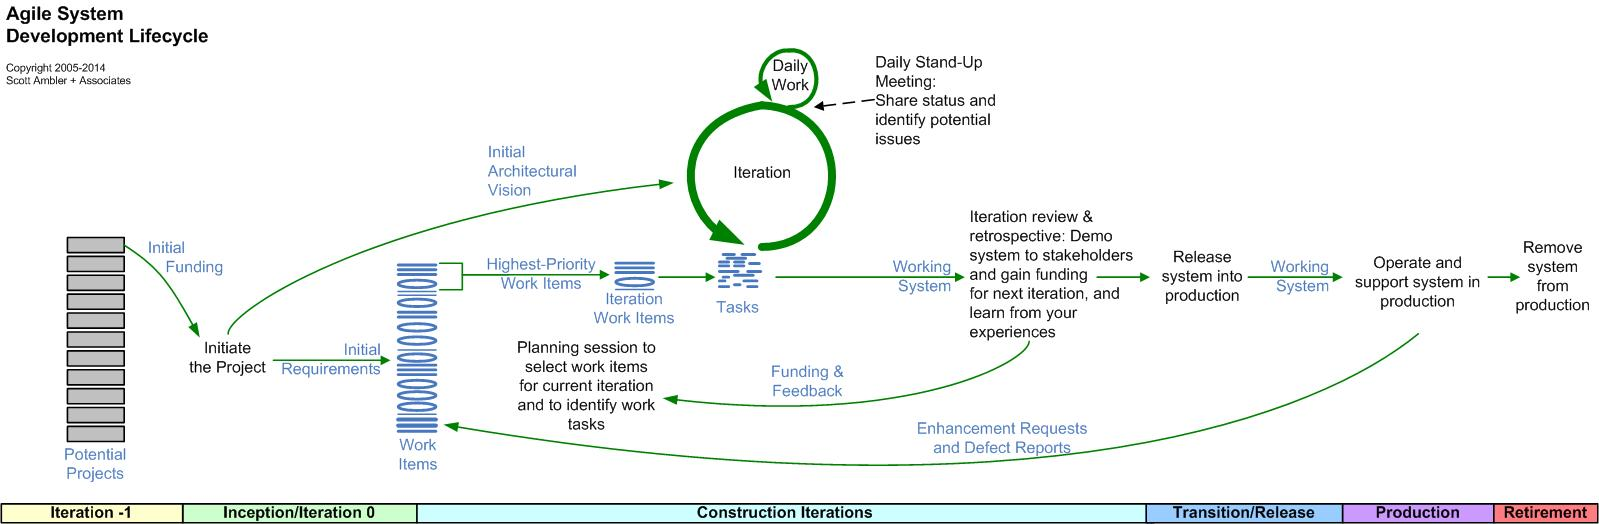
\includegraphics[width=1\textwidth]{lifecyclemodel/images/agileLifecycleDetailed} 
  \caption{Seleção do ciclo de vida ágil baseado no Scrum \cite{ambysoft:09}}
  \label{fig:scrumlifecycle} 
\end{figure}

\subsection{Análise dos requisitos do sistema}

\begin{itemize}
  \item Os requisitos serão definidos pelo fornecedor de acordo com as necessidades levantadas pelo adquirente

  \item Todos os requisitos serão definidos e listados no Product Backlog

  \item Eles serão listados e priorizados pelo PO (Product Owner) e Scrum Master antes do Sprint Planning
\end{itemize}

\subsection{Projeto de arquitetura do sistema}

Mais simples possível, segundo o manifesto ágil \cite{beck2001agile, BecAnd04extreme}. Simplicidade é:
\emph{"A arte de maximizar a quantidade de trabalho não feito."}


\subsection{Análise dos requisitos do software}

O trabalho a ser feito durante o Sprint é definido durante o Sprint Planning juntamente com todo o time de Scrum. No Sprint Planning é definido quais itens serão entregues no próximo Sprint. Estes itens são definidos de acordo com o Product Owner

\subsection{Projeto da arquitetura do sistema}

Manter mais simples possível. A arquitetura deve ser fácil para extender e modificá-la \cite{beck2001agile, BecAnd04extreme}.

\subsection{Projeto detalhado do software}

Mais simples possível para dar liberdade aos desenvolvedores \cite{beck2001agile, BecAnd04extreme}.

\subsection{Codificação e testes do software}

Programação pareada para funcionalidades complexas e TDD (Test driven development).

\subsection{Integração do software}

Integração contínua.

\subsection{Teste de qualificação do software}

Teste de integração ao final de cada sprint.

\subsection{Integração do sistema}

Integração contínua automatizada.

\subsection{Teste de qualificação do sistema}

Teste de acordo com os requisitos do sistema feitas pelo adquirente. Por exemplo, testar o cenário de aviso de pedidos prontos ao garçom num painel.

\subsection{Instalação do software}

Fornecedor irá prover manual de instalação.

\subsection{Apoio à aceitação do software}

O fornecedor irá prover treinamento ao adquirente.


\section{Processo de operação}
\label{sec:operacao}

Segundo a norma NBR ISO/IEC 12207:1998, o processo de operação é composto pelas seguintes atividades:

\begin{enumerate}
  \item Implementação do processo
  \item Teste operacional
  \item Operação do sistema
  \item Suporte ao usuário
\end{enumerate}

\subsection{Implementação do processo}

Para registrar, resolver e rastrear os problemas será utilizado o BugTracking. Problemas identificados serão incluídos no processo de resolução de problemas.%~\ref{sec:resolucao}.

\subsection{Teste operacional}

O teste será feito pelo desenvolvedor juntamente com o adquirente para liberação do produto de software.

\subsection{Operação do sistema}

Será disponibilizado um ambiente com as mesmas condições especificadas pelo adquirente para realizar os testes operacionais.

\subsection{Suporte ao usuário}

As solicitações do usuário, quando necessário, serão encaminhados para resolução no processo de manutenção.

\section{Processo de manutenção}
\label{sec:manutencao}

Segundo a norma NBR ISO/IEC 12207:1998, o processo de manutenção é composto pelas seguintes atividades:

\begin{enumerate}
  \item Implementação do processo
  \item Análise do problema e da modificação
  \item Implementação da modificação
  \item Revisão/aceitação da manutenção
  \item Migração
  \item Descontinuação do software
\end{enumerate}

\subsection{Implementação do processo}
Para registrar, resolver e rastrear os problemas será utilizado o BugTracking. Problemas identificados serão incluídos no processo de resolução de problemas. O gerenciamento do processo de manutenção será feito com Scrum.

\subsection{Análise do problema e da modificação}

O fornecedor fará a análise do problema e da modificação pedida pelo usuário. De acordo com o problema, definirá o nível de criticidade e o prazo para modificar.

\subsection{Implementação da modificação}

Esta atividade será feita pelo desenvolvedor durante a resolução do problema.

\subsection{Revisão/aceitação da manutenção}

O fornecedor fará a revisão junto ao adquirente da modificação solicitada.

\subsection{Migração}

Não haverá migração, pois é um sistema novo.

\subsection{Descontinuação do software}

Caso haja uma descontinuação do software, todos os artefatos gerados durante o ciclo de vida do processo de software serão disponibilizados ao cliente, bem como manuais ou qualquer outro documento que o adquirente tenha requisitado em comum acordo.












         % associado ao arquivo: 'cap-conceitos.tex'
%% ------------------------------------------------------------------------- %%
\chapter{Requisitos}
\label{cap:requisitos}

Apresentação do Wanderlei, basicamente só acrescentar. 
%% ------------------------------------------------------------------------- %%
\chapter{Testes e gerência de configuração}
\label{cap:testeconfiguracao}

Apresentação do dia 07/Novembro
%% ------------------------------------------------------------------------- %%
\chapter{Qualidade e gerência de engenharia de software}
\label{cap:qualigerencia}

Apresentação do último grupo
%% ------------------------------------------------------------------------- %%
\chapter{Conclus?es}
\label{cap:conclusoes}

Texto texto texto texto texto texto texto texto texto texto texto texto texto
texto texto texto texto texto texto texto texto texto texto texto texto texto
texto texto texto texto texto texto\footnote{Exemplo de refer?cia para p?ina
Web: \url{www.vision.ime.usp.br/~jmena/stuff/tese-exemplo}}.

%------------------------------------------------------
\section{Considera?es Finais} 

Texto texto texto texto texto texto texto texto texto texto texto texto texto
texto texto texto texto texto texto texto texto texto texto texto texto texto
texto texto texto texto texto texto. 

%------------------------------------------------------
\section{Sugest?es para Pesquisas Futuras} 

Texto texto texto texto texto texto texto texto texto texto texto texto texto
texto texto texto texto texto texto texto texto texto texto texto texto texto
texto texto texto texto texto texto.

Finalmente, leia o trabalho de Uri Alon \cite{alon09:how} no qual apresenta-se
uma reflex? sobre a utiliza?o da Lei de Pareto para tentar definir/escolher
problemas para as diferentes fases da vida acad?ica.  A dire?o dos novos
passos para a continuidade da vida acad?ica deveriam ser discutidos com seu
orientador.
        % associado ao arquivo: 'cap-conclusoes.tex'



% ---------------------------------------------------------------------------- %
% Bibliografia
\backmatter \singlespacing   % espaçamento simples
\bibliographystyle{alpha-ime}% citação bibliográfica alpha
\bibliography{bibliografia}  % associado ao arquivo: 'bibliografia.bib'

\end{document}
